\documentclass[10pt,a4paper]{article}
\usepackage[utf8]{inputenc}
\usepackage[T1]{fontenc}
\usepackage{geometry,amsmath,longtable,graphicx,pdfpages,hyperref}
\geometry{margin=1.7cm}
\hypersetup{colorlinks=true,linkcolor=blue,urlcolor=blue}
\setlength{\parindent}{0pt}
\setlength{\parskip}{0.45em}
\title{KFParticle $\Lambda$--$^{4}\mathrm{He}$\\Low / High Invariant-Mass CF Comparison}
\author{Post-processing QA report}
\date{2026-10-03 20:19 JST}
\begin{document}
\maketitle
\section{Sample, scope and common choices}
Au+Au fixed-target sample, beam-energy label 3.85 GeV; 2021 P24iy only. The beam label is not $\sqrt{s_{NN}}$. Partial merge: 26,956/26,994 subjobs; 38 excluded or missing.
Input: {\small\path{auau3p85_anaFemtoLambda_4He_KFParticle_2021P24iy_partial_merge.root}}. No event reanalysis, selection-cut change or original ROOT modification.
$k^*$ bin width: 20 MeV/$c$; display: $0$--$0.3$ GeV/$c$; normalization: $0.4$--$0.6$ GeV/$c$. The normalization interval remains in use even outside the displayed range.
The integrated comparison uses $0\leq k^*<0.2$ GeV/$c$. It is the normalized ratio of summed counts, not an arithmetic average of CF points. Each mass window is independently normalized.
\section{Inclusive 0--80\% comparison}
Ratios compare each half to full within the same background method. NA means unavailable, not zero or agreement. Errors are approximate (see limitations below).
\begin{itemize}
\item Raw: low/full = $1.001\pm0.00606$; high/full = $0.9992\pm0.00748$.
\item SBsub: low/full = $1.001\pm0.00644$; high/full = $0.9984\pm0.00805$.
\item CFsub: low/full = $1.001\pm0.00625$; high/full = $0.9986\pm0.0078$.
\item Method 3: low/full = NA; high/full = NA.
\item Method 5: low/full = $1\pm0.00607$; high/full = $0.9998\pm0.00803$.
\end{itemize}\section{Mass windows and methods}
Exact gates use candidate masses. Mass-fit projections and inclusive purity use whole stored mass bins, without split-bin interpolation:
\begin{center}\begin{tabular}{lcc}\hline Window & Exact nominal edges & Whole-bin edges\\\hline
full & 1.10708--1.12484 & 1.107--1.125\\
low & 1.10708--1.11596 & 1.107--1.116\\
high & 1.11596--1.12484 & 1.116--1.125\\
leftSB & 1.08044--1.10708 & 1.08--1.107\\
rightSB & 1.12484--1.15148 & 1.125--1.151\\
\hline\end{tabular}\end{center}
Edges are in GeV/$c^2$. Exact low excludes the mean, exact high includes it; the full outer edges are included. Whole-bin intervals are disjoint and half-open. Raw/SBsub/CFsub signal histograms use exact gates, while Methods 3/5 include this documented mass-binning difference.
\begin{description}
\item[Raw] Normalized signal SE/ME, without background correction.
\item[SBsub] Subtract summed sideband counts from SE and ME before normalization, using $1/3$ for full and $1/6$ for each half. A locally flat background is assumed.
\item[CFsub] $C_r^{\rm corr}=[C_r-(1-P_r)C_{\rm SB}]/P_r$. Each window uses its own current inclusive purity proxy.
\item[Method 3] Fit each SE/ME mass projection with Gaussian plus quadratic, then form the normalized ratio of $N-B$. Low/high background integrals share one fit; full uses their sum.
\item[Method 5] Purity fits use 50 MeV/$c$ coarse bins and $W=2$ neighbors per side: interior window 250 MeV/$c$, truncated at edges. Each original 5 MeV/$c$ count receives the purity of its containing coarse bin, then contributes to the 20 MeV/$c$ CF bin. No fine-bin refit is performed. Full has its own window purity; its corrected yield need not equal the sum of corrected half yields.
\end{description}
\begin{center}\begin{tabular}{lcc}\hline Window & Inclusive purity proxy & Actual width factor\\\hline
full & $0.9672\pm2.14e-05$ & 0.3396226\\
low & $0.9716\pm1.91e-05$ & 0.1698113\\
high & $0.9612\pm2.68e-05$ & 0.1698113\\
\hline\end{tabular}\end{center}
These purity errors are not propagated into CFsub. These are inclusive proxies, not measured pair-, centrality- or momentum-dependent purities; sideband asymmetry and background-model systematics remain.
\clearpage\section{Integrated CF values and half/full ratios}
Valid bins lists full/low/high counts in the displayed interval. A partial curve does not guarantee that the complete integration interval is valid. Invalid bins are not silently removed from the requested integration.
{\scriptsize\setlength{\tabcolsep}{3pt}\begin{longtable}{lrrrrrl}
\hline Method & $C_{\rm full}$ & $C_{\rm low}$ & $C_{\rm high}$ & Low/Full & High/Full & Valid bins\\\hline\endhead
\multicolumn{7}{l}{\textbf{Centrality 0-80\%}}\\
Raw & $1.056\pm0.0071$ & $1.057\pm0.00956$ & $1.055\pm0.0106$ & $1.001\pm0.00606$ & $0.9992\pm0.00748$ & 15/15/15 of 15\\
SBsub & $1.053\pm0.00765$ & $1.054\pm0.0102$ & $1.051\pm0.0115$ & $1.001\pm0.00644$ & $0.9984\pm0.00805$ & 15/15/15 of 15\\
CFsub & $1.053\pm0.00737$ & $1.054\pm0.00985$ & $1.051\pm0.0111$ & $1.001\pm0.00625$ & $0.9986\pm0.0078$ & 15/15/15 of 15\\
Method 3 & NA & $1.065\pm0.0101$ & NA & NA & NA & 14/15/14 of 15\\
Method 5 & $1.054\pm0.00736$ & $1.055\pm0.00972$ & $1.054\pm0.0113$ & $1\pm0.00607$ & $0.9998\pm0.00803$ & 15/15/15 of 15\\
\hline
\multicolumn{7}{l}{\textbf{Centrality 20-80\%}}\\
Raw & $1.126\pm0.0231$ & $1.13\pm0.0315$ & $1.121\pm0.0341$ & $1.004\pm0.0189$ & $0.9958\pm0.0223$ & 15/15/15 of 15\\
SBsub & $1.144\pm0.0269$ & $1.148\pm0.0359$ & $1.139\pm0.0398$ & $1.004\pm0.0211$ & $0.9956\pm0.0254$ & 15/15/15 of 15\\
CFsub & $1.125\pm0.024$ & $1.13\pm0.0324$ & $1.12\pm0.0355$ & $1.004\pm0.0195$ & $0.9955\pm0.0232$ & 15/15/15 of 15\\
Method 3 & NA & NA & NA & NA & NA & 13/13/13 of 15\\
Method 5 & $1.162\pm0.0251$ & $1.169\pm0.0335$ & $1.154\pm0.0379$ & $1.005\pm0.0192$ & $0.9925\pm0.0243$ & 15/15/15 of 15\\
\hline
\multicolumn{7}{l}{\textbf{Centrality 0-20\%}}\\
Raw & $1.049\pm0.00747$ & $1.05\pm0.01$ & $1.048\pm0.0112$ & $1.001\pm0.0064$ & $0.9993\pm0.00794$ & 15/15/15 of 15\\
SBsub & $1.045\pm0.00799$ & $1.046\pm0.0106$ & $1.043\pm0.012$ & $1.001\pm0.00676$ & $0.9986\pm0.0085$ & 15/15/15 of 15\\
CFsub & $1.046\pm0.00775$ & $1.047\pm0.0104$ & $1.044\pm0.0117$ & $1.001\pm0.0066$ & $0.9988\pm0.00828$ & 15/15/15 of 15\\
Method 3 & NA & $1.057\pm0.0106$ & NA & NA & NA & 14/15/14 of 15\\
Method 5 & $1.046\pm0.00771$ & $1.046\pm0.0102$ & $1.047\pm0.0118$ & $0.9997\pm0.00639$ & $1.001\pm0.0085$ & 15/15/15 of 15\\
\hline
\multicolumn{7}{l}{\textbf{Centrality 0-10\%}}\\
Raw & $1.046\pm0.00827$ & $1.047\pm0.0111$ & $1.045\pm0.0124$ & $1.001\pm0.00709$ & $0.999\pm0.00882$ & 15/15/15 of 15\\
SBsub & $1.042\pm0.0088$ & $1.043\pm0.0117$ & $1.04\pm0.0132$ & $1.002\pm0.00747$ & $0.9982\pm0.00941$ & 15/15/15 of 15\\
CFsub & $1.043\pm0.00859$ & $1.045\pm0.0115$ & $1.041\pm0.0129$ & $1.001\pm0.00732$ & $0.9984\pm0.00921$ & 15/15/15 of 15\\
Method 3 & NA & NA & NA & NA & NA & 14/14/14 of 15\\
Method 5 & $1.043\pm0.00851$ & $1.043\pm0.0112$ & $1.045\pm0.0131$ & $0.9993\pm0.00707$ & $1.001\pm0.00943$ & 15/15/15 of 15\\
\hline
\multicolumn{7}{l}{\textbf{Centrality 10-20\%}}\\
Raw & $1.076\pm0.0177$ & $1.079\pm0.0239$ & $1.074\pm0.0264$ & $1.002\pm0.0149$ & $0.9982\pm0.0182$ & 15/15/15 of 15\\
SBsub & $1.08\pm0.0194$ & $1.083\pm0.0259$ & $1.078\pm0.029$ & $1.002\pm0.016$ & $0.9977\pm0.0198$ & 15/15/15 of 15\\
CFsub & $1.075\pm0.0184$ & $1.078\pm0.0247$ & $1.073\pm0.0275$ & $1.002\pm0.0154$ & $0.9979\pm0.0189$ & 15/15/15 of 15\\
Method 3 & NA & NA & NA & NA & NA & 13/13/13 of 15\\
Method 5 & $1.087\pm0.0186$ & $1.091\pm0.0246$ & $1.084\pm0.0283$ & $1.003\pm0.0149$ & $0.997\pm0.0195$ & 15/15/15 of 15\\
\hline
\multicolumn{7}{l}{\textbf{Centrality 20-60\%}}\\
Raw & $1.126\pm0.0232$ & $1.132\pm0.0315$ & $1.121\pm0.0341$ & $1.005\pm0.0189$ & $0.9949\pm0.0223$ & 15/15/15 of 15\\
SBsub & $1.144\pm0.0269$ & $1.15\pm0.036$ & $1.138\pm0.0398$ & $1.005\pm0.0211$ & $0.9946\pm0.0254$ & 15/15/15 of 15\\
CFsub & $1.126\pm0.024$ & $1.131\pm0.0325$ & $1.12\pm0.0355$ & $1.005\pm0.0195$ & $0.9946\pm0.0232$ & 15/15/15 of 15\\
Method 3 & NA & NA & NA & NA & NA & 13/13/13 of 15\\
Method 5 & $1.155\pm0.025$ & $1.161\pm0.0334$ & $1.146\pm0.0378$ & $1.006\pm0.0192$ & $0.9922\pm0.0244$ & 15/15/15 of 15\\
\hline
\end{longtable}}
\section{Validity and uncertainty limitations}
An invalid fit in a required normalization bin makes its entire CF unavailable. Invalid comparison bins make the integrated contrast NA, not zero. Numerical convergence does not prove mass-model adequacy: large chi-square/ndf or small fit probabilities prohibit precision-model claims. Detailed fit diagnostics and NA reasons are in the Japanese README and extraction JSON.
First-order propagation retains shared full/half counts, sidebands, normalization integrals, the low/high background covariance from each common fit, and reuse of one coarse-bin purity by multiple CF bins. It cannot recover event / track sharing or mixed-pair reuse correlations. Covariance between observed $N$ and fitted background $B$, covariance between overlapping fits in different coarse bins, CFsub purity uncertainty and model systematics are not included. These comparisons are QA contrasts, not final significance tests.
Centrality groups overlap and are not independent. Low/high CFs cannot be directly added. Small TH2F rounding residuals are recorded without silently replacing the full histogram.
\section{Figure guide}
The next ten pages show two pages per method: Raw, SBsub, CFsub, Method 3, Method 5. First page: 0--80\%, 20--80\%, 0--20\%; second: 0--10\%, 10--20\%, 20--60\%. Upper panels: full (black), low (red), high (blue). Lower panels: low/full and high/full with supplied covariance errors. Failed bins are omitted, not displayed as measured zero.
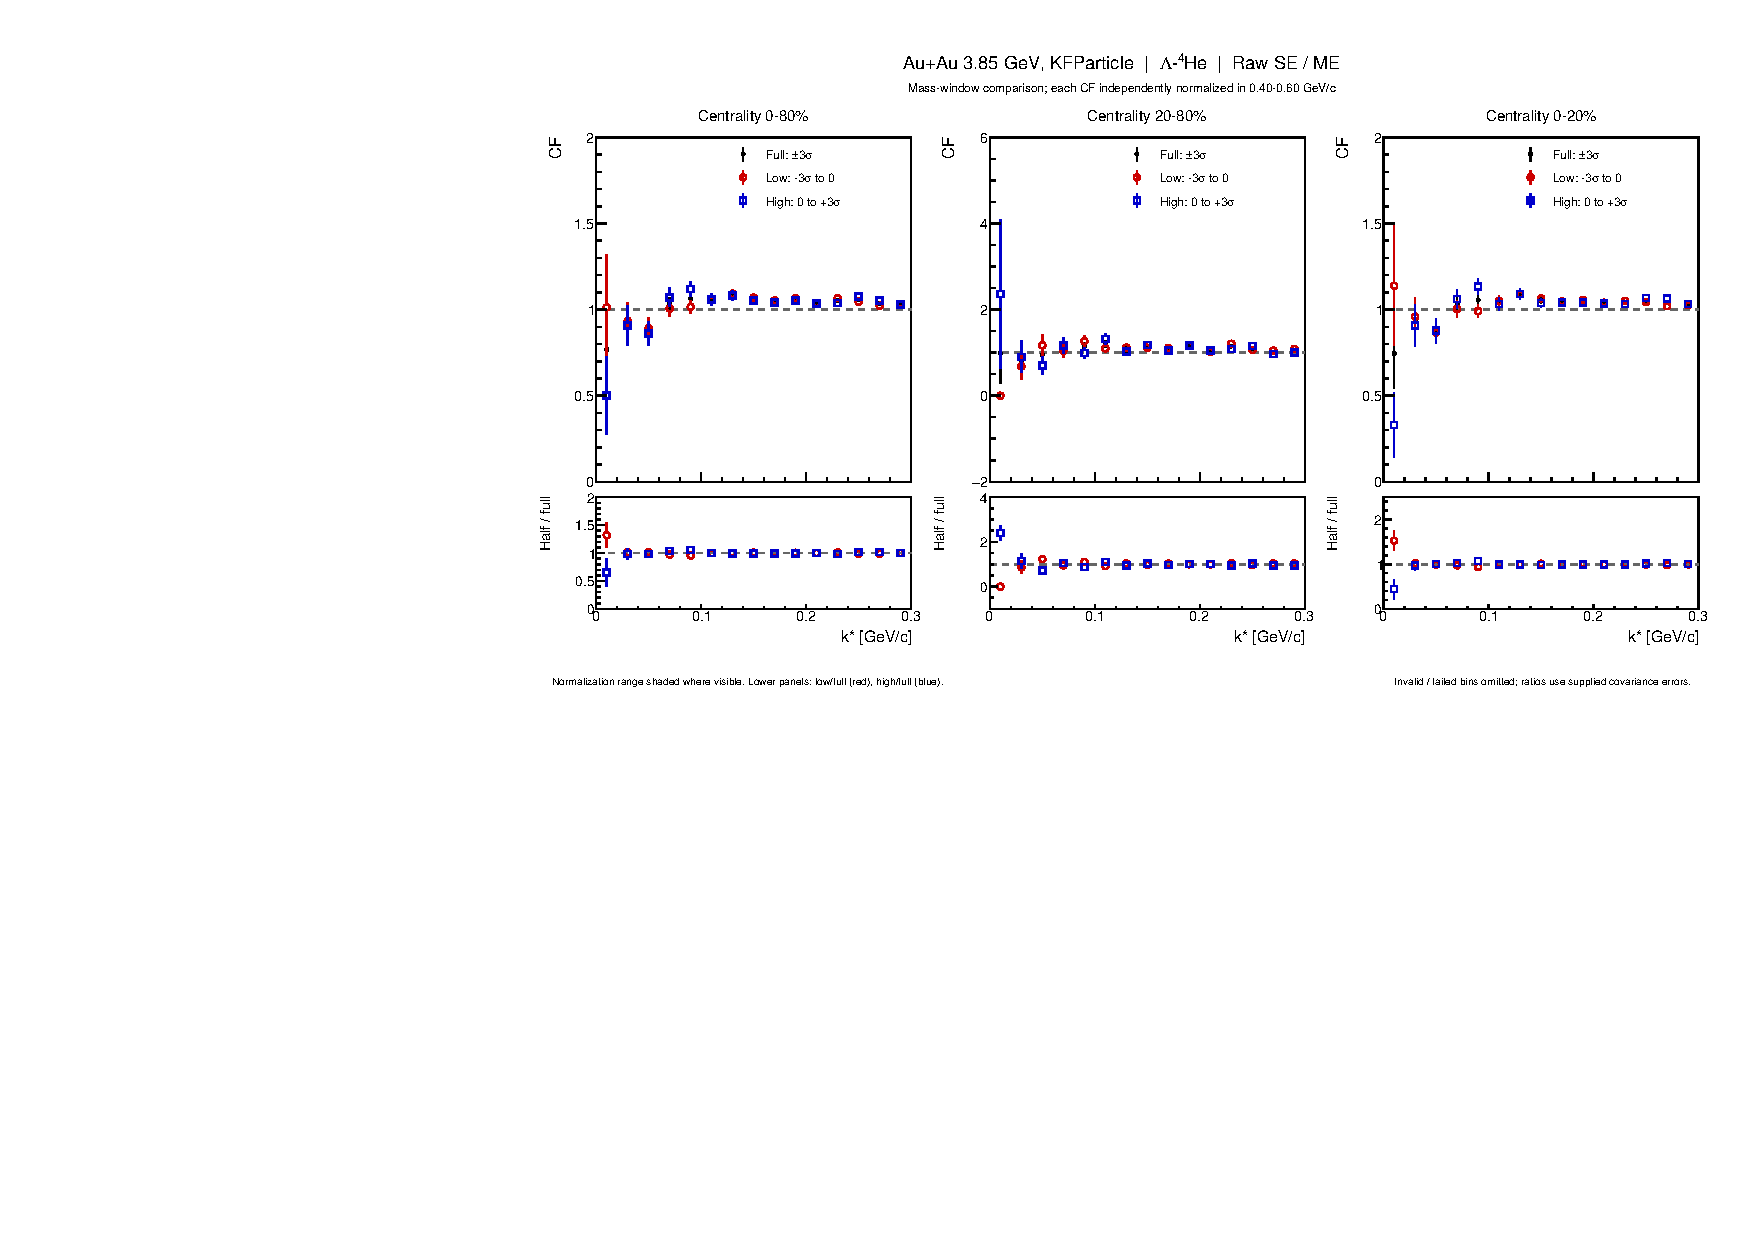
\includepdf[pages=-,fitpaper=true,pagecommand={}]{mass_halves_raw.pdf}
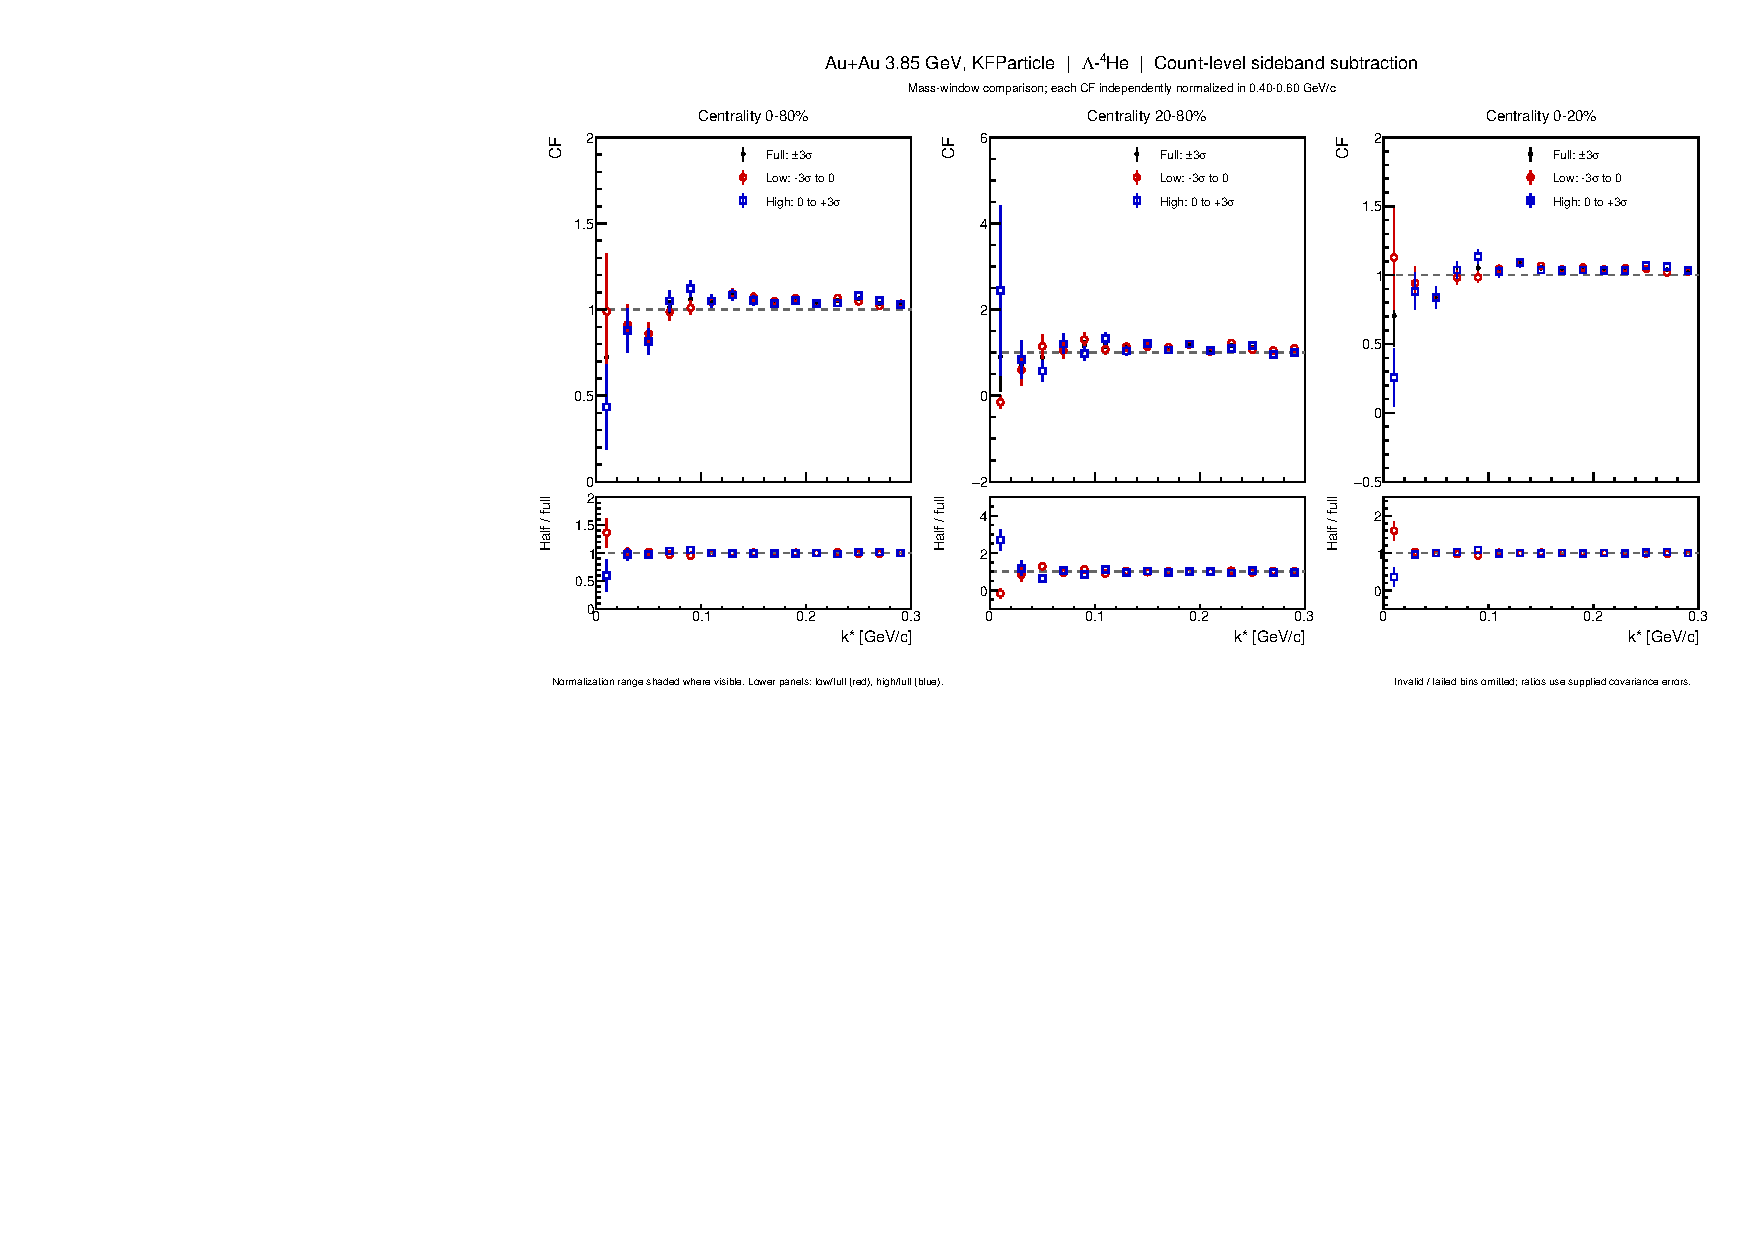
\includepdf[pages=-,fitpaper=true,pagecommand={}]{mass_halves_sbsub.pdf}
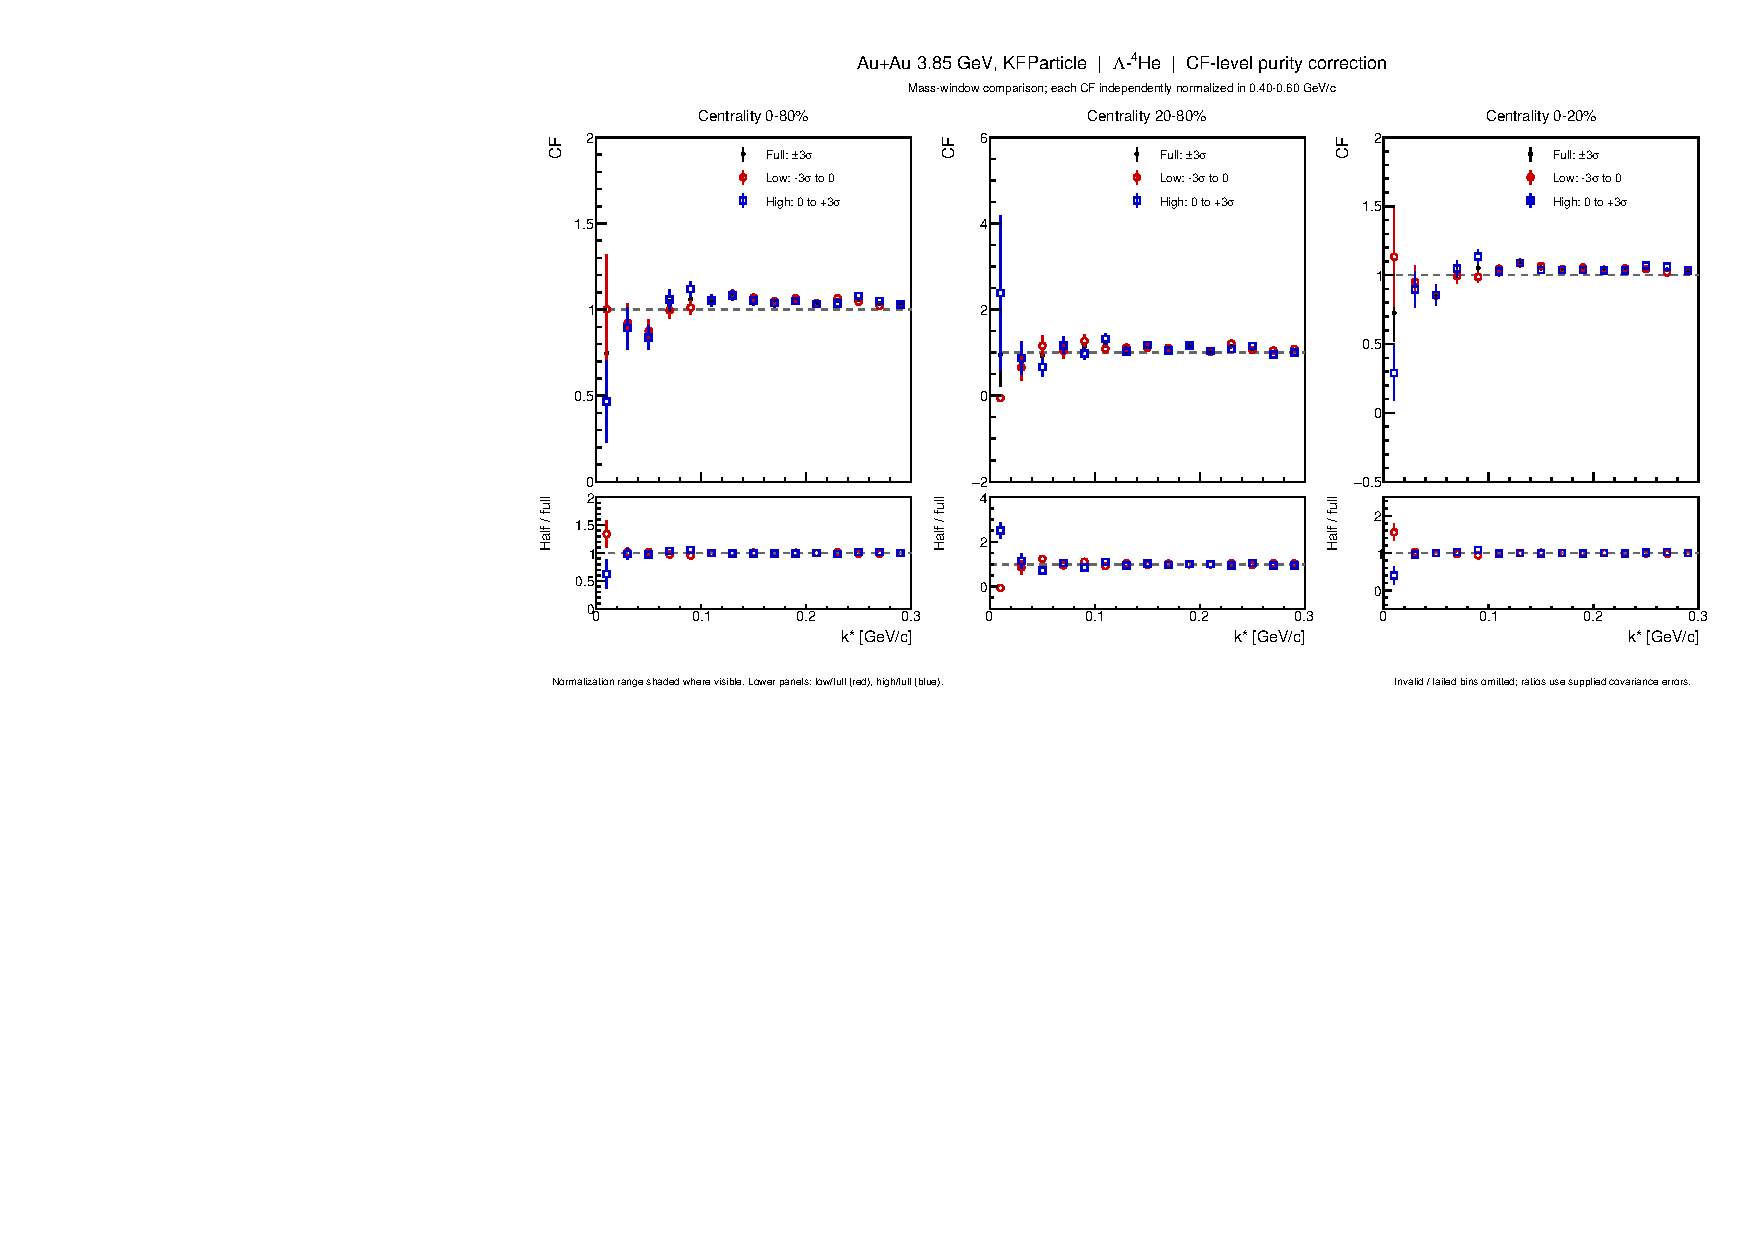
\includepdf[pages=-,fitpaper=true,pagecommand={}]{mass_halves_cfsub.pdf}
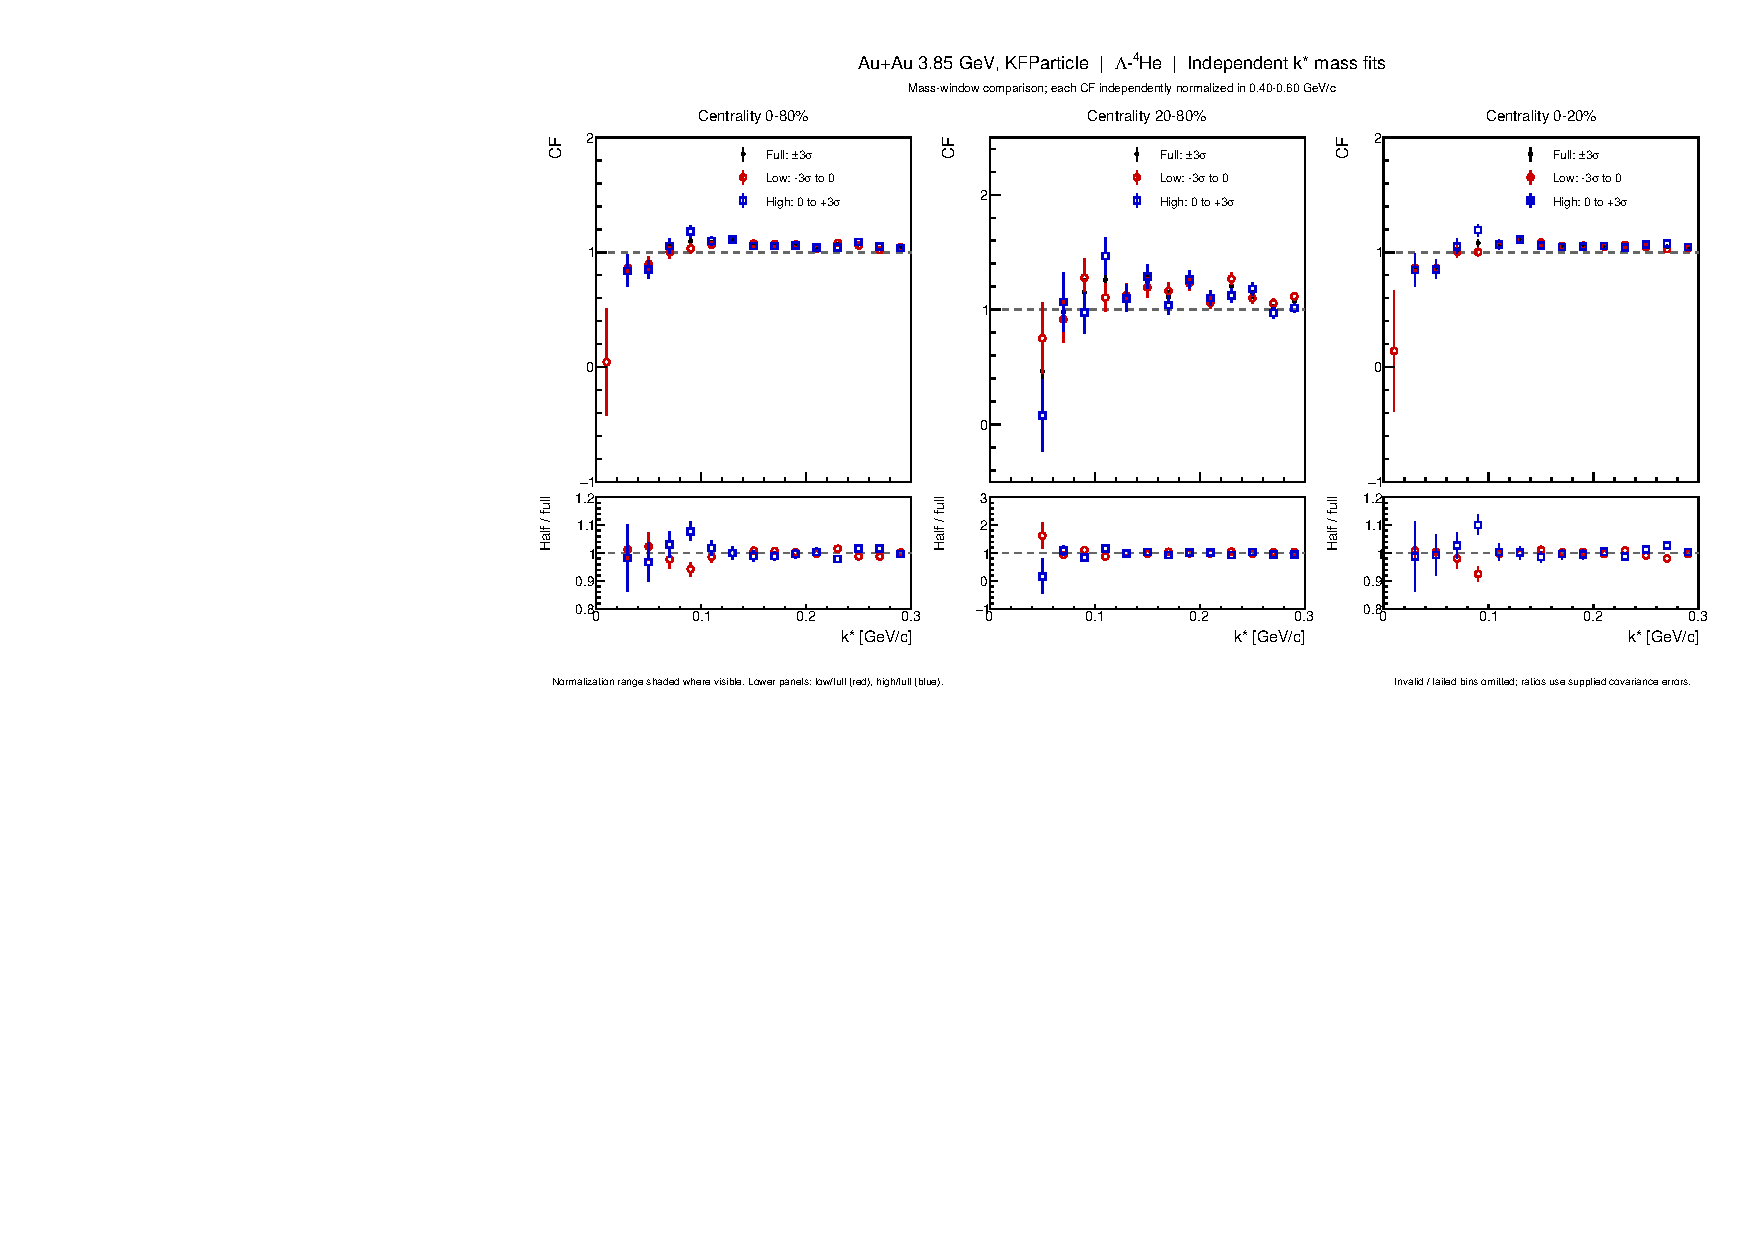
\includepdf[pages=-,fitpaper=true,pagecommand={}]{mass_halves_method3.pdf}
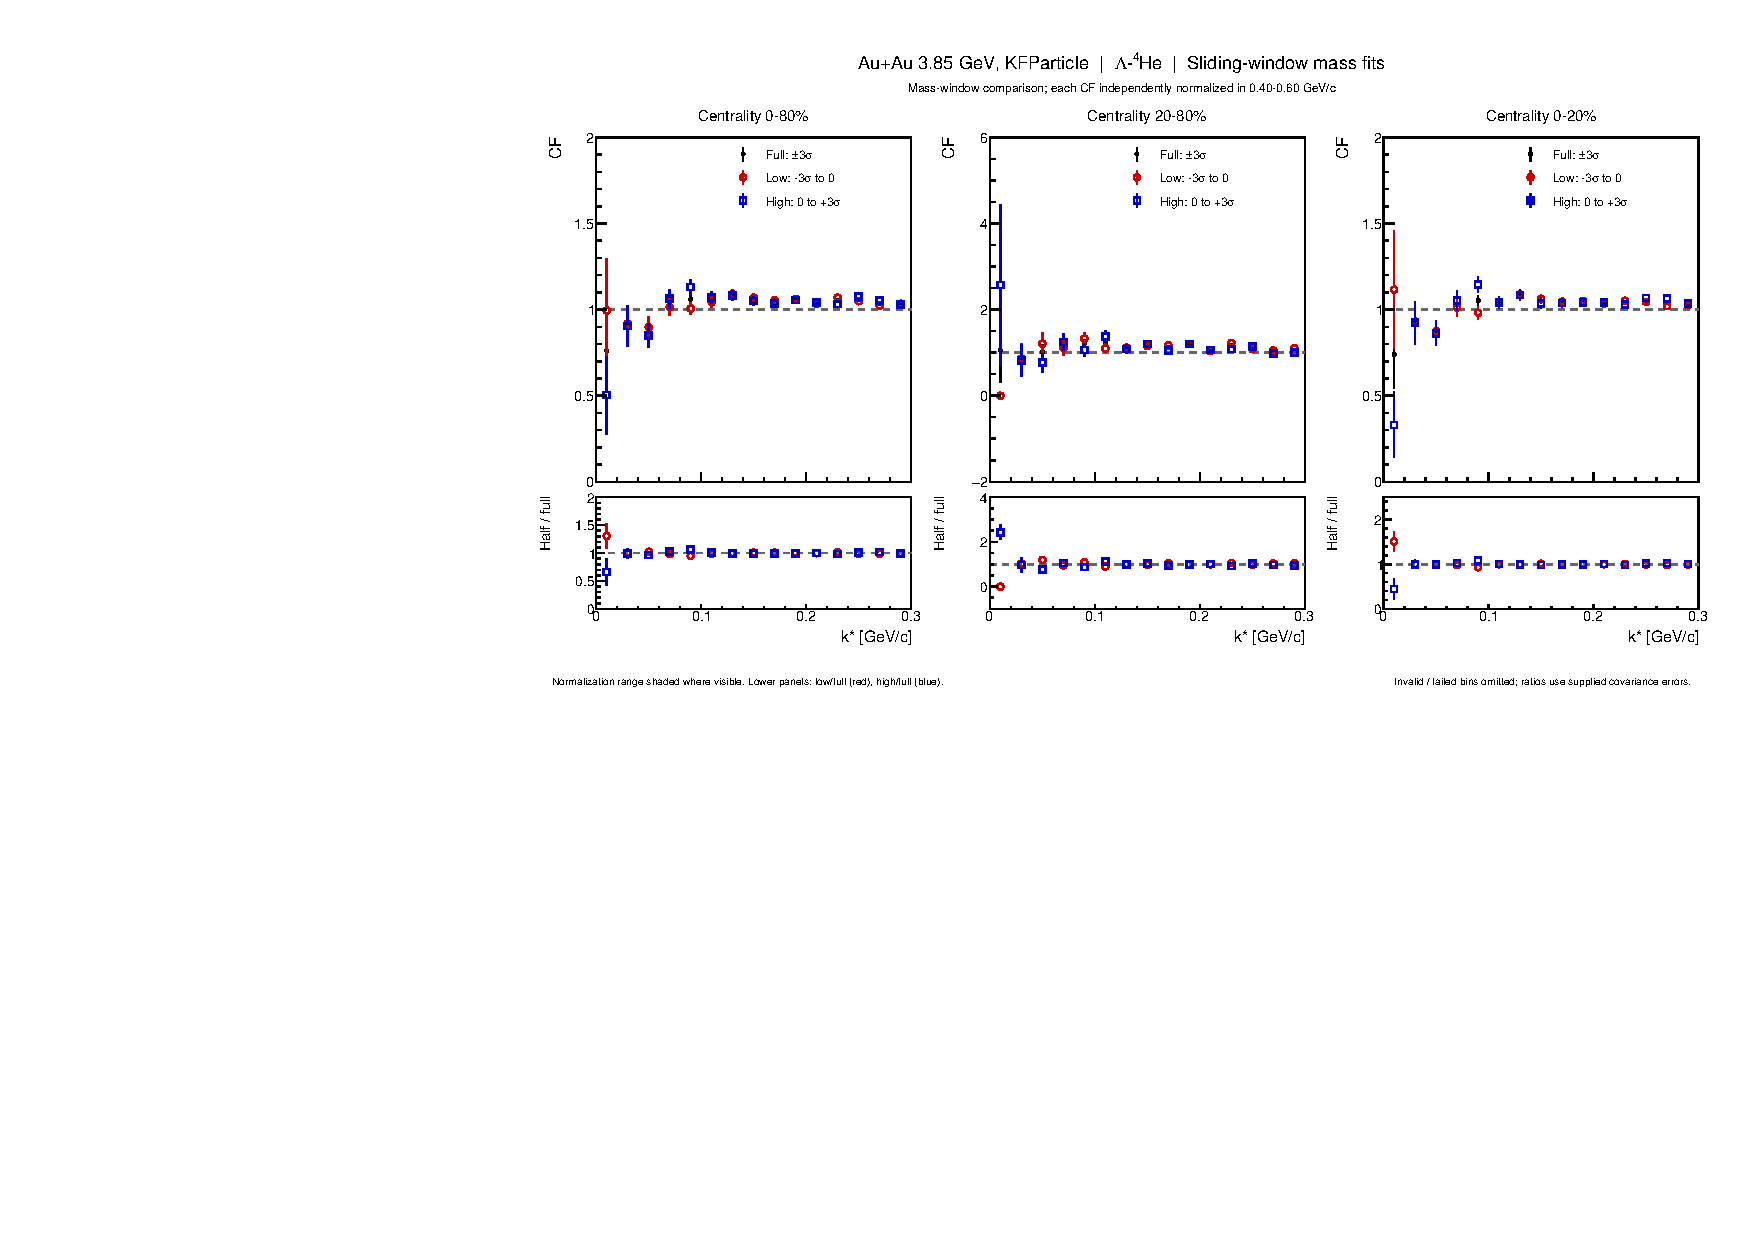
\includepdf[pages=-,fitpaper=true,pagecommand={}]{mass_halves_method5.pdf}
\end{document}
